\documentclass[12pt]{article}
\usepackage[margin=1in]{geometry}
\usepackage{amsmath,amssymb,amsthm,graphicx,booktabs}
\graphicspath{{../sims/out/}}
\newtheorem{proposition}{Proposition}
\setlength{\parindent}{0pt}\setlength{\parskip}{8pt}
\pagestyle{empty}
\begin{document}
\section*{Stein's core equations}

\textbf{Setup.} $X \sim N(\theta, \sigma^2 I_p)$, with $\theta$ unknown. Any estimator can be written as $\hat\theta = X + g(X)$.

\subsection*{1. Stein's lemma}
\[
\mathbb{E}\big[(X_i-\theta_i)\,g_i(X)\big] \;=\; \sigma^2\,\mathbb{E}\!\left[\frac{\partial g_i(X)}{\partial X_i}\right]
\]
The left side involves the unknown $\theta$. The right side needs only a derivative of $g$, which is computable from the data.

\subsection*{2. SURE (Stein's Unbiased Risk Estimate)}
\[
\mathbb{E}\,\|\hat\theta-\theta\|^2 \;=\; \mathbb{E}\Big[\,
\underbrace{p\sigma^2}_{\text{risk of } X}
\;+\; \underbrace{\|g(X)\|^2}_{\text{how far you moved}}
\;+\; \underbrace{2\sigma^2 \sum_i \frac{\partial g_i(X)}{\partial X_i}}_{\text{cross term, via Stein's lemma}}
\Big]
\]
Everything inside the brackets is computable from $X$, so it is an unbiased estimate of the risk.

\subsection*{3. The version that carries over to the thesis}
Before applying Stein's lemma, the same identity reads
\[
\mathbb{E}\,\|\hat\theta-\theta\|^2 \;=\; \mathbb{E}\,\|\hat\theta - X\|^2 \;-\; p\sigma^2 \;+\; 2\sum_i \operatorname{Cov}(\hat\theta_i, X_i)
\]
Substitute $X \to S$ and $\theta \to \Sigma$:
\[
\mathbb{E}\,\|\hat\Sigma-\Sigma\|_F^2 \;=\; \mathbb{E}\,\|\hat\Sigma - S\|_F^2 \;-\; \sum_{i,j}\operatorname{Var}(s_{ij}) \;+\; 2\sum_{i,j} \operatorname{Cov}(\hat\sigma_{ij}, s_{ij})
\]
This is Yi \& Zou's Lemma 1. Stein's lemma is what turns the Cov term into a derivative, and that step requires Gaussian data.

\newpage
\section*{Ledoit--Wolf shrinkage}

\textbf{The problem.} You want a $p\times p$ covariance matrix $\Sigma$ from $T$ observations.
The sample covariance $S$ is unbiased, but when $p$ is comparable to $T$ it is very noisy: the large
eigenvalues come out too large, the small ones too small, and the inverse is unstable. A structured
target $F$ (for example the identity times a scalar) has little noise but is biased. LW combine the two.

\textbf{The estimator.}
\[
\hat\Sigma \;=\; \delta F + (1-\delta) S, \qquad 0\le\delta\le 1
\]
The \emph{shrinkage intensity} $\delta$ is the knob. It is the same idea as James--Stein: pull a noisy
unbiased estimate toward a simple target, and accept a little bias for a large cut in variance.

\textbf{The loss.} Frobenius risk, i.e.\ total squared error over all $p^2$ entries:
\[
R(\delta) = \mathbb{E}\,\|\hat\Sigma - \Sigma\|_F^2 = \sum_{i,j}\mathbb{E}\big(\hat\sigma_{ij}-\sigma_{ij}\big)^2
\]

\subsection*{1. The optimal intensity (exact, finite sample)}
Each entry's error is variance plus squared bias. Using $\mathbb{E}s_{ij}=\sigma_{ij}$ and
$\phi_{ij}=\mathbb{E}f_{ij}$, minimizing $R(\delta)$ gives
\[
\delta^* \;=\; \frac{\displaystyle\sum_{i,j}\Big[\operatorname{Var}(s_{ij}) - \operatorname{Cov}(f_{ij},s_{ij})\Big]}
{\displaystyle\sum_{i,j}\Big[\operatorname{Var}(f_{ij}-s_{ij}) + (\phi_{ij}-\sigma_{ij})^2\Big]}
\;=\; \frac{\text{noise in } S \;-\; \text{co-movement of } F \text{ with } S}{\mathbb{E}\,\|F-S\|_F^2}
\]
\begin{itemize}
\item \textbf{Numerator:} how noisy $S$ is. More noise means shrink more. The Cov term subtracts the part
of the noise that $F$ shares with $S$, because $F$ is built from the same data and cannot cancel that part.
\item \textbf{Denominator:} how far apart $F$ and $S$ are, which includes the bias of the target
$(\phi_{ij}-\sigma_{ij})^2$. A badly wrong target means shrink less.
\end{itemize}
This $\delta^*$ is an \emph{oracle}: it depends on the unknown $\Sigma$.

\subsection*{2. LW's move: asymptotic approximation}
LW write $\delta^* \approx \kappa/T$ with
\[
\kappa = \frac{\pi - \rho}{\gamma}, \qquad
\pi = \sum_{i,j}\operatorname{AsyVar}(\sqrt T\, s_{ij}),\quad
\rho = \sum_{i,j}\operatorname{AsyCov}(\sqrt T\, f_{ij},\sqrt T\, s_{ij}),\quad
\gamma = \sum_{i,j}(\phi_{ij}-\sigma_{ij})^2
\]
and plug in \emph{consistent} estimators $\hat\pi,\hat\rho,\hat\gamma$ (with $\hat\gamma$ built from $\|F-S\|_F^2$):
\[
\hat\delta = \max\!\Big\{0,\ \min\!\Big\{\frac{\hat\kappa}{T},\,1\Big\}\Big\}
\]
\textbf{Targets.} LW (2003): single-index (market model) $F = s_m^2\,\hat\beta\hat\beta^\top + D$.
LW (2004): scaled identity $F=\nu I$ with $\nu=\operatorname{tr}S/p$, which gives the closed form
\[
\hat\delta_{\text{LW}} = \frac{\frac{1}{T^2}\sum_{t}\|x_tx_t^\top - S\|_F^2}{\|S-\nu I\|_F^2}
\]

\textbf{2004 intuition (a Pythagorean identity).} With $\mu = \operatorname{tr}\Sigma/p$,
\[
\underbrace{\mathbb{E}\|S-\mu I\|^2}_{d^2:\ \text{spread of } S}
= \underbrace{\|\Sigma-\mu I\|^2}_{a^2:\ \text{true spread}}
+ \underbrace{\mathbb{E}\|S-\Sigma\|^2}_{b^2:\ \text{estimation error}},
\qquad \delta^* = \frac{b^2}{d^2}
\]
The share of $S$'s apparent dispersion that is pure noise is exactly how much to shrink.

\subsection*{3. Link to Stein and to the thesis}
Plug $\hat\Sigma=\delta F+(1-\delta)S$ into the covariance form of SURE (page 1, eq.~3):
\[
R(\delta) = \delta^2\,\mathbb{E}\|F-S\|_F^2 + (1-2\delta)\sum_{i,j}\operatorname{Var}(s_{ij}) + 2\delta\sum_{i,j}\operatorname{Cov}(f_{ij},s_{ij})
\]
Its minimizer is exactly LW's $\delta^*$ above. So LW and SURE describe the \emph{same} risk curve.
\begin{center}
\begin{tabular}{l|l}
\textbf{Ledoit--Wolf} & \textbf{SURE (thesis)}\\\hline
estimate the three terms \emph{consistently} ($T\to\infty$) & estimate them \emph{unbiasedly} (any $T$)\\
gives one number $\hat\delta$ & gives the whole curve $\widehat R(\delta)$\\
Cov term via asymptotics & Cov term exact when $F$ is linear in $S$
\end{tabular}
\end{center}
The thesis question: does finite-sample unbiasedness beat asymptotic consistency when $T$ is small
relative to $p$, and what happens for targets (single-index) where the Cov term has no unbiased estimate?

\newpage
\section*{Two Stein shrinkers, worked through SURE}
Same setup as page 1: $X\sim N(\theta,\sigma^2I_p)$, $\hat\theta=X+g(X)$.

\subsection*{1. Linear shrinkage, $\hat\theta=(1-\lambda)X$}
Here $g=-\lambda X$ and $\sum_i\partial g_i/\partial X_i=-\lambda p$, so
\[
\mathrm{SURE}(\lambda)=p\sigma^2+\lambda^2\|X\|^2-2\lambda p\sigma^2,\qquad
\hat\lambda=\frac{p\sigma^2}{\|X\|^2}.
\]
The true risk is $R(\lambda)=(1-\lambda)^2p\sigma^2+\lambda^2\|\theta\|^2$, minimized at
$\lambda^*=p\sigma^2/(p\sigma^2+\|\theta\|^2)$. Since $\mathbb{E}\|X\|^2=p\sigma^2+\|\theta\|^2$,
$\hat\lambda$ is a plug-in ratio for $\lambda^*$, the same shape as $\hat\delta$ vs.\ $\delta^*$ on page 2.

\subsection*{2. James--Stein, $\hat\theta=\big(1-c/\|X\|^2\big)X$}
Here $\sum_i\partial g_i/\partial X_i=-c(p-2)/\|X\|^2$, so
\[
\mathrm{SURE}(c)=p\sigma^2+\frac{c^2-2c(p-2)\sigma^2}{\|X\|^2},
\]
minimized at $c=(p-2)\sigma^2$, giving $\mathrm{SURE}=p\sigma^2-(p-2)^2\sigma^4/\|X\|^2<p\sigma^2$ for
$p\ge3$. So James--Stein beats $X$ for every $\theta$. At $\theta=0$ (with $\sigma=1$) its risk is
$p-(p-2)^2\,\mathbb{E}[1/\chi^2_p]=2$.

\begin{center}
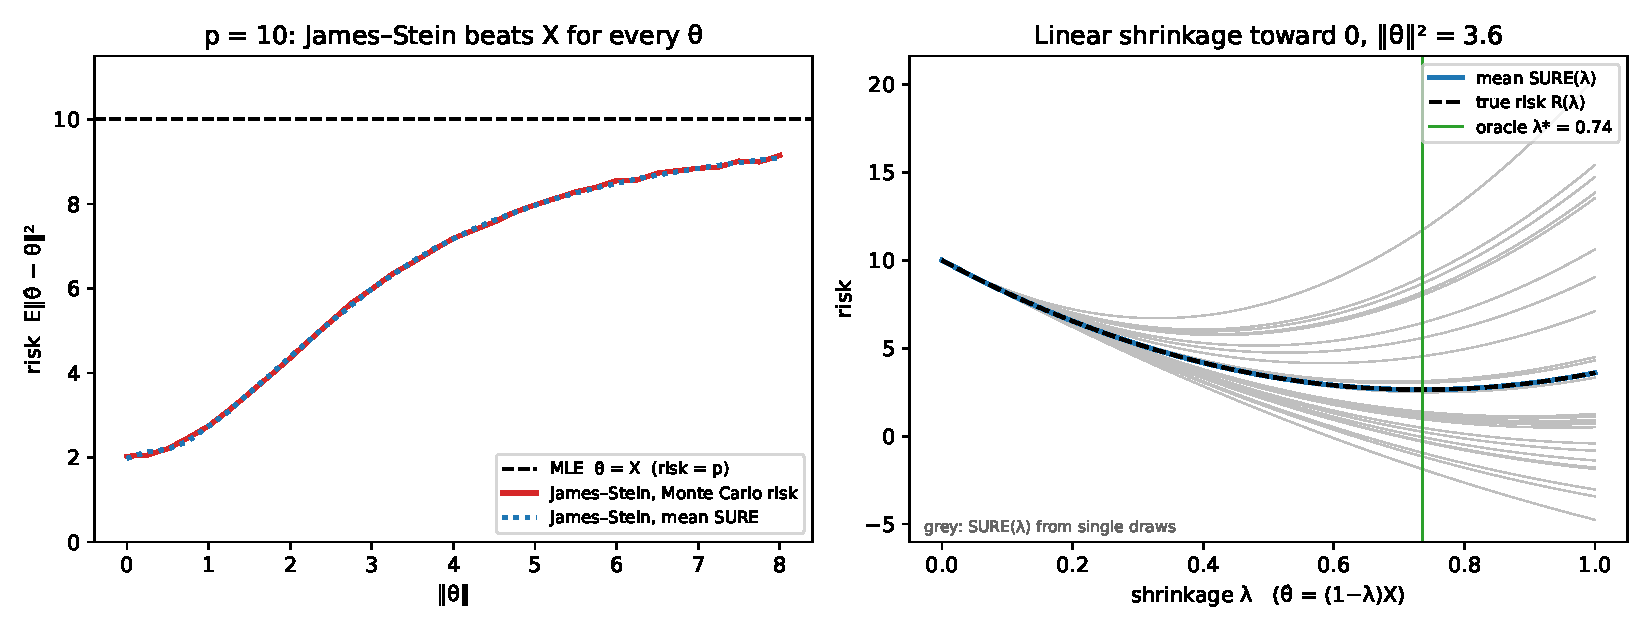
\includegraphics[width=\textwidth]{fig_stein.pdf}
\end{center}
\textit{Figure} (\texttt{sims/stein\_js.py}, $p=10$, $\sigma=1$). Left: risk of the MLE and of
James--Stein as $\|\theta\|$ grows, with the mean SURE of James--Stein. Right: SURE$(\lambda)$ for
linear shrinkage from single draws (grey), its mean, and the true risk.

\newpage
\section*{Deriving the three-piece formula, step by step}
\textbf{Goal.} Show that for \emph{any} estimate $\hat\Sigma$, if $\mathbb{E}S=\Sigma$,
\[
\mathbb{E}\|\hat\Sigma-\Sigma\|_F^2
=\underbrace{\mathbb{E}\|\hat\Sigma-S\|_F^2}_{\text{(a)}}
-\underbrace{V}_{\text{(b)}}
+\underbrace{2\sum_{i,j}\operatorname{Cov}(\hat\sigma_{ij},s_{ij})}_{\text{(c)}},
\qquad V=\sum_{i,j}\operatorname{Var}(s_{ij}).
\]

\subsection*{Step 1. Turn the matrix norm into a sum of numbers}
The squared Frobenius norm is the sum of squared entries, $\|A\|_F^2=\sum_{i,j}a_{ij}^2$. So
\[
\mathbb{E}\|\hat\Sigma-\Sigma\|_F^2=\sum_{i,j}\mathbb{E}\big(\hat\sigma_{ij}-\sigma_{ij}\big)^2 .
\]
From here on, fix one entry $(i,j)$ and drop the subscripts: write $\hat\sigma,\ s,\ \sigma$. We only
need to handle one number at a time, then add up.

\subsection*{Step 2. Add and subtract $s$}
\[
\hat\sigma-\sigma=\underbrace{(\hat\sigma-s)}_{\text{we can see this}}+\underbrace{(s-\sigma)}_{\text{noise in }s}
\]
This is the whole trick: split the unknown error into a part we observe and the noise of the data.

\subsection*{Step 3. Square it}
Using $(u+w)^2=u^2+w^2+2uw$:
\[
(\hat\sigma-\sigma)^2=(\hat\sigma-s)^2+(s-\sigma)^2+2(\hat\sigma-s)(s-\sigma).
\]

\subsection*{Step 4. Take expectations, term by term}
\begin{itemize}
\item First term: $\mathbb{E}(\hat\sigma-s)^2$. Keep it as is. Summed over $(i,j)$ this is (a).
\item Second term: $\mathbb{E}(s-\sigma)^2=\operatorname{Var}(s)$, \emph{because} $\mathbb{E}s=\sigma$ (variance is the
expected squared distance from the mean). This is the first place we use $\mathbb{E}S=\Sigma$.
\item Third term: the cross term $2\,\mathbb{E}\big[(\hat\sigma-s)(s-\sigma)\big]$, handled in Step 5.
\end{itemize}

\subsection*{Step 5. Simplify the cross term}
Split it in two:
\[
\mathbb{E}\big[(\hat\sigma-s)(s-\sigma)\big]=\mathbb{E}\big[\hat\sigma\,(s-\sigma)\big]-\mathbb{E}\big[s\,(s-\sigma)\big].
\]
\textbf{Why $\mathbb{E}[\hat\sigma(s-\sigma)]=\operatorname{Cov}(\hat\sigma,s)$.} Start from the definition of covariance
for any two random numbers $A$ and $B$:
\[
\operatorname{Cov}(A,B)=\mathbb{E}\big[(A-\mathbb{E}A)(B-\mathbb{E}B)\big].
\]
Multiply out the first bracket:
\[
\operatorname{Cov}(A,B)=\mathbb{E}\big[A\,(B-\mathbb{E}B)\big]-\mathbb{E}A\cdot\underbrace{\mathbb{E}\big[B-\mathbb{E}B\big]}_{=\,\mathbb{E}B-\mathbb{E}B\,=\,0}
=\mathbb{E}\big[A\,(B-\mathbb{E}B)\big].
\]
($\mathbb{E}A$ is a constant, so it comes out of the expectation.) In words: to get a covariance you only
need to centre \emph{one} of the two variables; centring the other adds a term with mean zero.
Now take $A=\hat\sigma$ and $B=s$. Since $\mathbb{E}s=\sigma$, the centred $B$ is exactly $s-\sigma$:
\[
\operatorname{Cov}(\hat\sigma,s)=\mathbb{E}\big[\hat\sigma\,(s-\mathbb{E}s)\big]=\mathbb{E}\big[\hat\sigma\,(s-\sigma)\big].
\]
This is where $\mathbb{E}S=\Sigma$ is needed: if $\mathbb{E}s\neq\sigma$, then $s-\sigma$ is not centred and the
identity picks up an extra $\mathbb{E}\hat\sigma\cdot(\mathbb{E}s-\sigma)$. Note that $\hat\sigma$ itself never needs to be
centred, and $\hat\sigma$ can be biased, data-dependent, anything.

\textbf{Why $\mathbb{E}[s(s-\sigma)]=\operatorname{Var}(s)$.} Same identity with $A=s$:
$\mathbb{E}[s(s-\sigma)]=\operatorname{Cov}(s,s)=\operatorname{Var}(s)$.
So the cross term is $2\operatorname{Cov}(\hat\sigma,s)-2\operatorname{Var}(s)$. This is the second place we use $\mathbb{E}S=\Sigma$.

\subsection*{Step 6. Put the pieces back together}
\[
\mathbb{E}(\hat\sigma-\sigma)^2
=\mathbb{E}(\hat\sigma-s)^2+\operatorname{Var}(s)+2\operatorname{Cov}(\hat\sigma,s)-2\operatorname{Var}(s)
=\mathbb{E}(\hat\sigma-s)^2-\operatorname{Var}(s)+2\operatorname{Cov}(\hat\sigma,s).
\]
Summing over all $(i,j)$ gives exactly (a) $-$ (b) $+$ (c). \hfill$\square$

\subsection*{What the derivation used, and what it did not}
\begin{itemize}
\item \textbf{Used:} only $\mathbb{E}S=\Sigma$, in Steps 4 and 5. This is why the open issue about dividing by $T$
vs.\ $T-1$ (and the unknown mean) matters: if $\mathbb{E}S\neq\Sigma$, a bias term appears.
\item \textbf{Not used:} any distribution (no normality), and nothing about the form of $\hat\Sigma$. It holds for
LW, for tapering (Yi \& Zou), for any estimator.
\item \textbf{Stein's version} is the same six steps with $X,\theta,\hat\theta$ in place of $S,\Sigma,\hat\Sigma$. Stein then
adds one more step that needs normality: $\operatorname{Cov}(\hat\theta_i,X_i)=\sigma^2\,\mathbb{E}[\partial\hat\theta_i/\partial X_i]$.
The thesis replaces that step with U-statistics (pages 8--9).
\end{itemize}

\newpage
\section*{The covariance version, in plain words}

\textbf{The idea in one line.} We want to know how wrong our covariance estimate $\hat\Sigma$ is, but the
truth $\Sigma$ is unknown. Stein's trick, carried over to matrices, rewrites ``how wrong'' using only
things the data can tell us.

\subsection*{1. Split the error into three pieces}
For any estimate $\hat\Sigma$, as long as $S$ is right on average ($\mathbb{E}S=\Sigma$):
\[
\underbrace{\mathbb{E}\|\hat\Sigma-\Sigma\|_F^2}_{\text{how wrong we are}}
=\underbrace{\mathbb{E}\|\hat\Sigma-S\|_F^2}_{\text{(a) how far we moved from }S}
\;-\;\underbrace{V}_{\text{(b) noise in }S}
\;+\;\underbrace{2\sum_{i,j}\operatorname{Cov}(\hat\sigma_{ij},s_{ij})}_{\text{(c) how much we copy that noise}}
\]
\begin{itemize}
\item[(a)] Observable: we can compute $\|\hat\Sigma-S\|_F^2$ directly.
\item[(b)] $V=\sum_{ij}\operatorname{Var}(s_{ij})=\mathbb{E}\|S-\Sigma\|_F^2$, the error of the raw sample
covariance. It is subtracted because part of (a) is just $S$ being noisy, not us being wrong.
\item[(c)] The penalty. If $\hat\Sigma$ follows every random wiggle in $S$, it inherits $S$'s error; if it
ignores $S$, it inherits none.
\end{itemize}

\textbf{Two sanity checks.}
\begin{itemize}
\item Use $\hat\Sigma=S$ (no shrinkage): (a) $=0$ and (c) $=2V$, so the error is $0-V+2V=V$. Correct: the
error of $S$ is its own noise.
\item Use a fixed $\hat\Sigma=F$ that ignores the data: (c) $=0$, so the error is $\mathbb{E}\|F-S\|^2-V=\|F-\Sigma\|^2$.
Correct: a fixed guess is wrong by exactly its distance from the truth.
\end{itemize}

\subsection*{2. Plug in Ledoit--Wolf shrinkage}
With $\hat\Sigma=\delta F+(1-\delta)S$, the three pieces become
\[
R(\delta)=\delta^2D+(1-2\delta)V+2\delta C,
\]
where each letter is a single number:
\begin{center}
\begin{tabular}{@{}lll@{}}
\toprule
Symbol & Definition & In words \\
\midrule
$D$ & $\mathbb{E}\|F-S\|_F^2$ & how far the target is from the data \\
$V$ & $\sum_{ij}\operatorname{Var}(s_{ij})$ & how noisy the sample covariance is \\
$C$ & $\sum_{ij}\operatorname{Cov}(f_{ij},s_{ij})$ & how much the target moves with that noise \\
\bottomrule
\end{tabular}
\end{center}
$R(\delta)$ is a parabola in $\delta$. Its lowest point is $\delta^*=(V-C)/D$: shrink more when $S$ is
noisy ($V$ large), less when the target is far off ($D$ large) or shares $S$'s noise ($C$ large).
SURE replaces $D,V,C$ by estimates from the data; that gives an estimated parabola we can minimize.

\textbf{Why it is true (short proof; full walk-through on pages 5--6).} Write the error as $(\hat\Sigma-S)+(S-\Sigma)$ and square. The
squares give (a) and $V$; the cross term, using $\mathbb{E}s_{ij}=\sigma_{ij}$, is
$2\sum\operatorname{Cov}(\hat\sigma_{ij},s_{ij})-2V$. That is the three-piece formula. For LW,
$\hat\Sigma-S=\delta(F-S)$ gives (a) $=\delta^2D$, and
$\operatorname{Cov}(\hat\sigma_{ij},s_{ij})=\delta\operatorname{Cov}(f_{ij},s_{ij})+(1-\delta)\operatorname{Var}(s_{ij})$
gives (c) $=2\delta C+2(1-\delta)V$. Adding: $\delta^2D-V+2\delta C+2(1-\delta)V=\delta^2D+(1-2\delta)V+2\delta C$. \hfill$\square$

\subsection*{3. Side by side with Stein}
Same formula, different objects:
\begin{center}
\small
\begin{tabular}{@{}lll@{}}
\toprule
 & Stein: estimate a mean & Thesis: estimate a covariance \\
\midrule
Seen / wanted & $X$ / $\theta$ & $S$ / $\Sigma$ \\
Right on average & $\mathbb{E}X=\theta$ & $\mathbb{E}S=\Sigma$ \\
(b) noise in the raw estimate & $p\sigma^2$ & $V$ \\
(a) how far we moved & $\|\hat\theta-X\|^2$ & $\delta^2\|F-S\|_F^2$ \\
(c) copy-the-noise penalty & $2\sum_i\operatorname{Cov}(\hat\theta_i,X_i)$ & $2\sum_{ij}\operatorname{Cov}(\hat\sigma_{ij},s_{ij})$ \\
How (c) is estimated & Stein's lemma (normal data only) & pairs of days (any data) \\
Shrink rule & $(1-\lambda)X$ & $\delta F+(1-\delta)S$ \\
Data-chosen amount & $\hat\lambda=p\sigma^2/\|X\|^2$ & $\hat\delta=(\hat V-\hat C)/\|F-S\|_F^2$ \\
\bottomrule
\end{tabular}
\end{center}

\subsection*{4. Where the thesis departs from Stein}
\textbf{Stein's way needs normal data.} Stein's lemma turns the penalty (c) into a derivative, but only
when the data follow a bell curve. Every earlier way of estimating $V$ and $C$ inherits that
assumption: the Stein--Haff identity (Haff, 1980), Yi \& Zou's Lemma~2, and RBLW (Chen et al., 2010).
Stock returns have fat tails, so this matters.

\textbf{The thesis way: count, don't assume.} Both $V$ and $C$ are just combinations of fourth moments
(here $X_t$ is day $t$'s return vector, mean known to be zero, $S=\frac1T\sum_tX_tX_t^\top$):
\[
V=\frac{\mathbb{E}\|X\|^4-\operatorname{tr}\Sigma^2}{T},\qquad
C=\frac{\operatorname{Var}(\|X\|^2)}{pT}=\frac{\mathbb{E}\|X\|^4-(\operatorname{tr}\Sigma)^2}{pT}\quad(F=\nu I).
\]
Each ingredient has a simple unbiased estimate:
\begin{center}
\begin{tabular}{@{}lll@{}}
\toprule
Estimate & Formula & What it averages \\
\midrule
$\hat M\to\mathbb{E}\|X\|^4$ & $\frac1T\sum_t\|X_t\|^4$ & each day's size, to the fourth power \\
$\hat U_2\to\operatorname{tr}\Sigma^2$ & $\frac{1}{T(T-1)}\sum_{t\neq u}(X_t^\top X_u)^2$ & how alike two different days are \\
$\hat U_3\to(\operatorname{tr}\Sigma)^2$ & $\frac{1}{T(T-1)}\sum_{t\neq u}\|X_t\|^2\|X_u\|^2$ & size of one day times size of another \\
\bottomrule
\end{tabular}
\end{center}
Using pairs of \emph{different} days ($t\neq u$) is the key: different days are independent, so the
average of a product equals the product of averages, with no bias. Then
\[
\hat V=\frac{\hat M-\hat U_2}{T},\qquad \hat C=\frac{\hat M-\hat U_3}{pT}.
\]
These are right on average for any distribution with finite fourth moments. So the SURE curve is
exactly unbiased at every $\delta$ without assuming normality. The same works for the targets $I$
(where $C=0$) and $D_S$. It does \emph{not} work for single-index or constant-correlation, because
those targets are nonlinear in $S$.

\textbf{Does it matter in practice?} Yes. In the simulation ($p=100$, AR(1), $r=0.5$), SURE stays within
about 3\% of the best possible (oracle) error at every sample size, with normal or fat-tailed ($t_{10}$)
data. With fat tails, RBLW and OAS, which assume normality, are 1.2--4.6 times the oracle error.

\newpage
\section*{The role of Yi \& Zou's Lemma}
\subsection*{1. What the lemma says}
Yi \& Zou (2013), Lemma~1 (dissertation Lemma~2.2.1, eq.~2.6). For \emph{any} estimator $\hat\Sigma$,
\[
\mathbb{E}\|\hat\Sigma-\Sigma\|_F^2=\mathbb{E}\|\hat\Sigma-S\|_F^2-\sum_{i,j}\operatorname{Var}(s_{ij})+2\sum_{i,j}\operatorname{Cov}(\hat\sigma_{ij},s_{ij}).
\]
This is exactly the three-piece formula (a) $-$ (b) $+$ (c); pages 5--6 are its proof. Yi \& Zou define
$S=\frac{1}{n-1}\sum(X-\bar X)(X-\bar X)^\top$: the $n-1$ divisor with an estimated mean, chosen precisely
so that $\mathbb{E}S=\Sigma$ holds.

\subsection*{2. The role it plays}
\begin{enumerate}
\item \textbf{It swaps an unknown for knowns.} The usual bias--variance split,
\[
\mathbb{E}\|\hat\Sigma-\Sigma\|_F^2=\sum_{i,j}\operatorname{Var}(\hat\sigma_{ij})+\sum_{i,j}\big(\mathbb{E}\hat\sigma_{ij}-\sigma_{ij}\big)^2,
\]
contains the unknown $\sigma_{ij}$ in the bias term. Yi's form replaces it with $\mathbb{E}\|\hat\Sigma-S\|_F^2$, which
the data shows directly. That is what makes the risk estimable.
\item \textbf{It holds for any estimator.} Yi \& Zou apply it to tapering; the thesis applies it to
Ledoit--Wolf. Nothing needs re-deriving.
\item \textbf{It reduces the problem to two quantities}, $\operatorname{Var}(s_{ij})$ and
$\operatorname{Cov}(\hat\sigma_{ij},s_{ij})$. This is where the thesis and Yi \& Zou part ways:
\end{enumerate}
\begin{center}
\small
\begin{tabular}{@{}lll@{}}
\toprule
 & Yi \& Zou & Thesis \\
\midrule
Estimator & tapering, $\hat\sigma_{ij}=w_{ij}s_{ij}$ & LW, $\delta F+(1-\delta)S$ \\
$\operatorname{Var}(s_{ij})$ & Lemma 2.2.2: exact, normal data only & $(\hat M-\hat U_2)/T$, any distribution \\
Cov term & $w_{ij}\operatorname{Var}(s_{ij})$ (fixed weights) & needs $\operatorname{Cov}(f_{ij},s_{ij})$ ($F$ uses the data) \\
\bottomrule
\end{tabular}
\end{center}

\subsection*{3. Rewriting the Frobenius error with the lemma}
\textbf{Step 1: apply the lemma to LW.} With $\hat\Sigma=\delta F+(1-\delta)S$:
\begin{itemize}
\item (a): $\hat\Sigma-S=\delta(F-S)$, so $\mathbb{E}\|\hat\Sigma-S\|_F^2=\delta^2D$.
\item (c): $\operatorname{Cov}(\hat\sigma_{ij},s_{ij})=\delta\operatorname{Cov}(f_{ij},s_{ij})+(1-\delta)\operatorname{Var}(s_{ij})$, so (c) $=2\delta C+2(1-\delta)V$.
\end{itemize}
\[
\mathbb{E}\|\hat\Sigma-\Sigma\|_F^2=\delta^2D-V+2\delta C+2(1-\delta)V=\boxed{\delta^2D+(1-2\delta)V+2\delta C}.
\]
\textbf{Step 2: turn it into SURE.} The risk $R(\delta)=\delta^2D+(1-2\delta)V+2\delta C$ has three unknown
numbers, one per piece of the three-piece formula:
\begin{center}
\begin{tabular}{@{}lll@{}}
\toprule
Piece & Unknown & In words \\
\midrule
(a) how far we moved & $D=\mathbb{E}\|F-S\|_F^2$ & distance between target and data \\
(b) noise in $S$ & $V=\sum_{ij}\operatorname{Var}(s_{ij})$ & how much $S$ jumps around \\
(c) copying the noise & $C=\sum_{ij}\operatorname{Cov}(f_{ij},s_{ij})$ & how much the target jumps with $S$ \\
\bottomrule
\end{tabular}
\end{center}
SURE swaps each unknown for a number computed from the data that is right on average:
\[
\mathrm{SURE}(\delta)=\delta^2\hat D+(1-2\delta)\hat V+2\delta\hat C .
\]
Because $\delta$ is a fixed number we choose, $\mathbb{E}\,\mathrm{SURE}(\delta)=\delta^2\mathbb{E}\hat D+(1-2\delta)\mathbb{E}\hat V+2\delta\,\mathbb{E}\hat C=R(\delta)$.
So the whole job is three estimates. Below, each one: what it measures, how to compute it, why it is
right on average.

\subsubsection*{Setup}
The data are $T$ days of returns on $p$ assets. Day $t$ is a vector $X_t$ (one return per asset), the days
are independent, and the mean return is taken as $0$. Then
\[
S=\frac1T\sum_tX_tX_t^\top,\qquad \nu=\frac{\operatorname{tr}S}{p},\qquad F=\nu I .
\]
Two numbers per day or per pair of days are all we need:
\[
n_t=\|X_t\|^2\ \ (\text{size of day }t),\qquad g_{tu}=X_t^\top X_u\ \ (\text{overlap of days }t\text{ and }u).
\]

\subsubsection*{The one idea behind (b) and (c)}
A variance is ``mean of the square minus square of the mean'': $\operatorname{Var}(Y)=\mathbb{E}[Y^2]-(\mathbb{E}Y)^2$. From data:
\begin{itemize}
\item \textbf{Same-day products} ($Y_t\cdot Y_t$) average to $\mathbb{E}[Y^2]$, the mean of the square.
\item \textbf{Different-day products} ($Y_t\cdot Y_u$, $t\neq u$) average to $(\mathbb{E}Y)^2$, the square of the mean,
because independent days give $\mathbb{E}[Y_tY_u]=\mathbb{E}Y_t\cdot\mathbb{E}Y_u$.
\end{itemize}
So: (average over same-day products) $-$ (average over different-day products) is an unbiased variance.
Pieces (b) and (c) are this idea applied to two different $Y$'s.

\subsubsection*{Piece (a): $\hat D$}
\textbf{Measures:} how far the target is from the sample covariance.\\
\textbf{Compute:} $\hat D=\|F-S\|_F^2=\sum_{i,j}(f_{ij}-s_{ij})^2$.\\
\textbf{Right on average:} $D$ is \emph{defined} as the average of exactly this quantity, so nothing to prove.

\subsubsection*{Piece (b): $\hat V$}
\textbf{Measures:} the noise in $S$. Each day contributes the matrix $Y_t=X_tX_t^\top$, and $S$ is their average.
So $V$ is ``how much one day's matrix varies'', divided by $T$ (averaging $T$ independent days divides
variance by $T$):
\[
V=\frac1T\Big(\underbrace{\mathbb{E}\|Y\|_F^2}_{\text{mean of square}}-\underbrace{\|\mathbb{E}Y\|_F^2}_{\text{square of mean}}\Big)
=\frac1T\Big(\mathbb{E}\|X\|^4-\operatorname{tr}\Sigma^2\Big),
\]
since $\|Y\|_F^2=\|X\|^4$ and $\mathbb{E}Y=\Sigma$.\\
\textbf{Compute:} the matrix-version of ``product'' is $\langle Y_t,Y_u\rangle=g_{tu}^2$ (and $=n_t^2$ when $t=u$).
\[
\hat M=\frac1T\sum_tn_t^2\ \ (\text{same day}),\qquad
\hat U_2=\frac{1}{T(T-1)}\sum_{t\neq u}g_{tu}^2\ \ (\text{different days}),\qquad
\hat V=\frac{\hat M-\hat U_2}{T}.
\]
\textbf{Right on average:} $\mathbb{E}\hat M=\mathbb{E}\|X\|^4$; for $t\neq u$, independence gives $\mathbb{E}g_{tu}^2=\operatorname{tr}\Sigma^2$. So $\mathbb{E}\hat V=V$.

\subsubsection*{Piece (c): $\hat C$}
\textbf{Measures:} how much the target moves together with $S$. $F=\nu I$ is zero off the diagonal (no
movement there), and on the diagonal it is $\nu=\operatorname{tr}S/p$. Adding up the diagonal,
$C=\operatorname{Cov}(\nu,\operatorname{tr}S)=\operatorname{Var}(\operatorname{tr}S)/p$. Now $\operatorname{tr}S$ is the average of the daily sizes $n_t$, so
\[
C=\frac{1}{pT}\operatorname{Var}(n)=\frac{1}{pT}\Big(\underbrace{\mathbb{E}[n^2]}_{\text{mean of square}}-\underbrace{(\mathbb{E}n)^2}_{\text{square of mean}}\Big)
=\frac{1}{pT}\Big(\mathbb{E}\|X\|^4-(\operatorname{tr}\Sigma)^2\Big).
\]
\textbf{Compute:} same idea with $Y=n$, a single number per day:
\[
\hat M=\frac1T\sum_tn_t^2\ \ (\text{same day}),\qquad
\hat U_3=\frac{1}{T(T-1)}\sum_{t\neq u}n_tn_u\ \ (\text{different days}),\qquad
\hat C=\frac{\hat M-\hat U_3}{pT}.
\]
\textbf{Right on average:} $\mathbb{E}\hat M=\mathbb{E}\|X\|^4$; for $t\neq u$, $\mathbb{E}[n_tn_u]=\mathbb{E}n_t\,\mathbb{E}n_u=(\operatorname{tr}\Sigma)^2$. So $\mathbb{E}\hat C=C$.

\subsubsection*{Worked example by hand ($p=2$ assets, $T=4$ days)}
Days: $X_1=(1,1)$, $X_2=(-1,0)$, $X_3=(0,1)$, $X_4=(-1,-1)$.
\begin{enumerate}
\item \textbf{Sizes} $n_t$: $2,\,1,\,1,\,2$.
\item \textbf{Overlaps} $g_{tu}$ for the 6 pairs: $g_{12}=-1$, $g_{13}=1$, $g_{14}=-2$, $g_{23}=0$, $g_{24}=1$, $g_{34}=-1$.
\item $S=\frac14\sum_tX_tX_t^\top=\begin{pmatrix}3/4&1/2\\1/2&3/4\end{pmatrix}$, so $\nu=\frac{3/4+3/4}{2}=\frac34$ and
$F-S=\begin{pmatrix}0&-1/2\\-1/2&0\end{pmatrix}$.
\item \textbf{(a)} $\hat D=0+\tfrac14+\tfrac14+0=\tfrac12$.
\item \textbf{Same day:} $\hat M=\frac{4+1+1+4}{4}=\frac52$.
\item \textbf{(b) different days:} squares of overlaps $1+1+4+0+1+1=8$; each pair counts twice ($t,u$ and
$u,t$), so $\hat U_2=\frac{2\cdot8}{4\cdot3}=\frac43$, and $\hat V=\frac{5/2-4/3}{4}=\frac{7}{24}$.
\item \textbf{(c) different days:} products of sizes $2+2+4+1+2+2=13$, so $\hat U_3=\frac{2\cdot13}{12}=\frac{13}{6}$, and
$\hat C=\frac{5/2-13/6}{2\cdot4}=\frac{1}{24}$.
\item \textbf{SURE:} $\mathrm{SURE}(\delta)=\tfrac12\delta^2+(1-2\delta)\tfrac{7}{24}+2\delta\cdot\tfrac{1}{24}=\tfrac12\delta^2-\tfrac12\delta+\tfrac{7}{24}$.
\item \textbf{Best $\delta$:} $\hat\delta=\frac{\hat V-\hat C}{\hat D}=\frac{7/24-1/24}{1/2}=\frac12$, where SURE drops from $\frac{7}{24}$ (no
shrinkage) to $\frac16$.
\end{enumerate}

\subsubsection*{On a computer}
Form the $T\times T$ matrix $G=XX^\top$ (all overlaps; its diagonal is the sizes $n_t$). Then
$\sum_{t\neq u}g_{tu}^2=\sum_{t,u}G_{tu}^2-\sum_tn_t^2$ and $\sum_{t\neq u}n_tn_u=(\sum_tn_t)^2-\sum_tn_t^2$, so no loop over pairs is
needed. In simulation ($p=100$, $T=20$, 4000 datasets) the average SURE matches the average actual loss
at every $\delta$ (e.g.\ $\delta=0.5$: 143.7 vs.\ 143.6).

\textbf{Two cautions.}
\begin{itemize}
\item SURE is right on average at each \emph{fixed} $\delta$. The chosen $\hat\delta$ is a ratio of random numbers, so it is
not exactly right on average for the best $\delta^*$ (page~\pageref{pg:parallel}). If $\hat\delta$ falls outside $[0,1]$, clip it.
\item Nothing above assumed normal data: only independent days, mean $0$, and finite fourth moments.
\end{itemize}

\textbf{Step 3: compare with Yi's own case.} For tapering, $\hat\sigma_{ij}=w_{ij}s_{ij}$ with fixed weights, the same
steps give
\[
\mathrm{SURE}=\sum_{i,j}(1-w_{ij})^2s_{ij}^2+\sum_{i,j}(2w_{ij}-1)\widehat{\operatorname{Var}}(s_{ij}),
\]
which is their eq.~(2.11) up to an $(n-1)/n$ factor from how they scale $S$. LW toward $F=0$ is the special
case $w_{ij}=1-\delta$ for all $(i,j)$, with $C=0$.

\subsection*{4. A note on dropping $V$}
The $-V$ term is the same for every estimator, so Yi \& Zou drop it when only \emph{comparing} estimators
(their ``partial risk''). For LW, $V$ cannot be dropped entirely: it comes back through the Cov term via
$(1-\delta)\operatorname{Var}(s_{ij})$. That is why $V$ appears in $R(\delta)$ and in $\delta^*=(V-C)/D$.

\newpage
\section*{A parallel worth checking}\label{pg:parallel}
In both problems the data-driven intensity differs from a neighbouring estimator by a small finite-sample
correction:
\begin{itemize}
\item Normal means: linear SURE gives $\hat\lambda=p\sigma^2/\|X\|^2$; James--Stein uses $(p-2)\sigma^2/\|X\|^2$.
The $-2$ appears because James--Stein's SURE accounts for the intensity depending on $X$; plugging
$\hat\lambda$ into a fixed-$\lambda$ SURE does not.
\item Covariance: LW (2004) uses $\frac{T-1}{T}\hat V/\|F-S\|_F^2$; SURE uses $(\hat V-\hat C)/\|F-S\|_F^2$.
\end{itemize}
In both, SURE is unbiased for the risk at a fixed intensity, but the minimizer is a ratio of estimates and
is not unbiased for the oracle. Open question: does a SURE that accounts for $\hat\delta$ depending on $S$,
as James--Stein's does for $\hat\lambda$, give a further correction (the analogue of $p\to p-2$), and does it
lower risk at small $T$?

\newpage
\section*{Every piece of the thesis, mapped to Stein}
Each result from the work with Professor Rosenman has a direct counterpart in Stein's normal-means
problem. The table is the summary; the numbered items give the details (item 1 is derived on pages 5--6,
item 6 is on page 15).

\begin{center}
\small
\begin{tabular}{@{}p{0.31\textwidth}p{0.31\textwidth}p{0.3\textwidth}@{}}
\toprule
Thesis result & Stein counterpart & Status \\
\midrule
1. Risk in SURE form (Yi \& Zou Lemma 1) & Covariance-penalty form of SURE & Proved (pages 5--6, 10--11) \\
2. LW 2004 Pythagoras, $\delta^*=b^2/d^2$ & James--Stein as empirical Bayes & Same identity \\
3. $R(\delta)<R(0)$ iff $0<\delta<2\delta^*$ & JS dominates $X$ iff $0<c<2(p-2)\sigma^2$ & Proved, 2026-10-26 \\
4. $\delta^*\ge0$; clip $\hat\delta$ to $[0,1]$ & Positive-part James--Stein & Proved \\
5. Unbiased $\hat V,\hat C$ by U-statistics & Stein's lemma / Stein--Haff (Gaussian) & Proved for $\nu I$ \\
6. LW $=$ SURE minus finite-sample terms & $p$ vs.\ $p-2$ & Proved; $p-2$ analogue open \\
7. Gaussian check vs.\ Chen et al.\ eq.~(7) & Gaussian SURE / Rao--Blackwell & Checked \\
8. Touloumis (2015) comparison & ``Stein-type'' shrinkage, U-statistics & To do \\
9. Single-index target & Stein's lemma on a nonlinear $F$ & Open (target decision) \\
10. Simulations & \texttt{stein\_js.py} & Done for $\nu I$ \\
\bottomrule
\end{tabular}
\end{center}

\subsection*{2. LW's Pythagoras is James--Stein's empirical-Bayes identity}
Normal means: $\mathbb{E}\|X\|^2=\|\theta\|^2+p\sigma^2$, i.e.\ $d^2=a^2+b^2$ with $a^2=\|\theta\|^2$ (true
spread) and $b^2=p\sigma^2$ (noise). The oracle linear intensity is
\[
\lambda^*=\frac{p\sigma^2}{p\sigma^2+\|\theta\|^2}=\frac{b^2}{d^2},
\]
exactly LW (2004)'s $\delta^*=b^2/d^2$ on page 3. In the empirical-Bayes reading (Efron \& Morris), with
$\theta\sim N(0,\tau^2I)$ the Bayes shrinkage factor is $\sigma^2/(\sigma^2+\tau^2)$, and
$(p-2)\sigma^2/\|X\|^2$ is an unbiased estimate of it. LW estimate $b^2/d^2$ consistently; the thesis
estimates the numerator and denominator unbiasedly.

\subsection*{3. The risk-reduction window is the James--Stein window}
\begin{itemize}
\item Linear normal means: $R(\lambda)-R(0)=\lambda\big[\lambda(p\sigma^2+\|\theta\|^2)-2p\sigma^2\big]<0$ iff
$0<\lambda<2\lambda^*$.
\item James--Stein: $\mathrm{SURE}(c)-p\sigma^2=\big(c^2-2c(p-2)\sigma^2\big)/\|X\|^2<0$ iff $0<c<2(p-2)\sigma^2$.
\item Thesis: $R(\delta)-R(0)=\delta\big[\delta D-2(V-C)\big]<0$ iff $0<\delta<2\delta^*$, $\delta^*=(V-C)/D$.
\end{itemize}
All three are the same quadratic: any shrinkage up to twice the optimum beats no shrinkage. The window is
set by the oracle; the estimated version $0<\delta<2\hat\delta$ only describes the estimated curve.

\subsection*{4. $\delta^*\ge0$ and clipping are the positive-part story}
$V\ge C$ by Cauchy--Schwarz on $\operatorname{tr}S$ (\texttt{sure\_scaled\_identity.pdf}), so $\delta^*\ge0$:
shrinking toward $\nu I$ never makes the oracle want to push \emph{away} from the target. But
$\hat\delta=(\hat V-\hat C)/\|F-S\|^2$ can fall outside $[0,1]$, which is why LW clip it. That is the
positive-part James--Stein estimator $\big(1-(p-2)\sigma^2/\|X\|^2\big)_+X$, which strictly improves on
plain James--Stein (Baranchik, 1964). Clipping $\hat\delta$ should likewise only help, but it makes the
SURE of the clipped rule no longer exactly the fixed-$\delta$ formula.

\subsection*{5. Unbiased terms: Stein's lemma vs.\ U-statistics}
Stein estimates the covariance penalty by integration by parts, which needs the Gaussian density; its
Wishart version (Stein--Haff) underlies Yi \& Zou Lemma~2 and RBLW. The thesis gets the same three terms
from moments: $\hat V=(\hat M-\hat U_2)/T$ and $\hat C=(\hat M-\hat U_3)/(pT)$ are unbiased under finite
fourth moments alone. Monte Carlo agrees (\texttt{sims/out/results.txt}): e.g.\ $t_{10}$, $p=100$, $T=40$:
$V=340.24$ vs.\ mean $\hat V=339.16$ (MC s.e.\ $0.86$); $C=0.944$ vs.\ $0.939$ (s.e.\ $0.006$).

\subsection*{7. The Gaussian check}
Under Gaussian data the distribution-free decomposition gives an $\alpha^*$ identical to Chen et al.\ eq.~(7),
the oracle that RBLW estimates by Rao--Blackwellizing LW. So the thesis SURE contains the Gaussian
Stein-world answer as a special case and drops the assumption it rests on. This is visible in the
simulation: under Gaussian data SURE $\approx$ OAS; under $t_{10}$ RBLW and OAS lose because they hard-code the
Gaussian fourth moment.

\subsection*{8. Touloumis is ``Stein-type'' in the James--Stein sense}
Touloumis (2015) titles the estimators ``nonparametric Stein-type'': James--Stein-style linear shrinkage
toward $\nu I$, $I$, or $D_S$, with $\operatorname{tr}\Sigma^2$ and $\operatorname{tr}^2\Sigma$ estimated by
unbiased U-statistics ($Y_{1N}$, $Y_{2N}$). That is the closest existing estimator to the thesis; the
difference is that the thesis targets the finite-sample risk curve rather than a ratio-consistent
intensity. The head-to-head comparison is still to do. Schäfer \& Strimmer (2005), next on the reading
list, is also James--Stein-type with term-by-term estimates.

\subsection*{9. Single-index target: where Stein's lemma could come back}
For $F$ nonlinear in $S$ (single-index, constant-correlation) no unbiased moment estimate of $C$ is
available. Under Gaussian data, Stein's lemma gives a route. With $x_t\sim N(0,\Sigma)$ and
$\mathbb{E}[x_{ti}h(X)]=\sum_k\sigma_{ik}\,\mathbb{E}[\partial h/\partial x_{tk}]$, taking $h=x_{tj}f_{ij}$,
\[
\operatorname{Cov}(f_{ij},\,x_{ti}x_{tj})=\sum_k\sigma_{ik}\,\mathbb{E}\Big[x_{tj}\,\frac{\partial f_{ij}}{\partial x_{tk}}\Big],
\]
and $\operatorname{Cov}(f_{ij},s_{ij})$ is the average over $t$. This still involves $\Sigma$, so plugging in
$S$ gives an \emph{approximate} SURE, not an exact one. This is a concrete option for the target decision
to raise with Professor Rosenman: exact distribution-free SURE for linear targets, or Gaussian
approximate SURE for single-index.

\subsection*{10. The simulations side by side}
\begin{center}
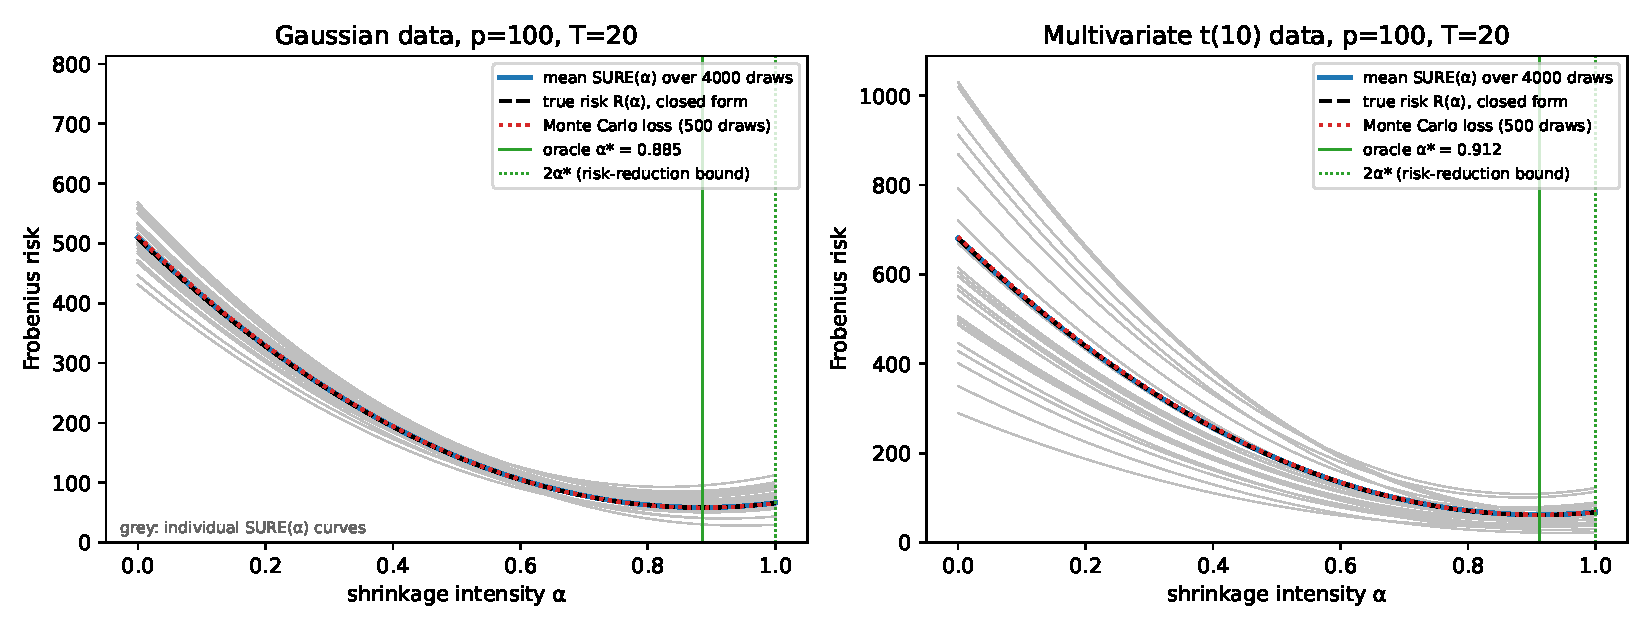
\includegraphics[width=0.49\textwidth]{fig_sure_vs_risk.pdf}\hfill
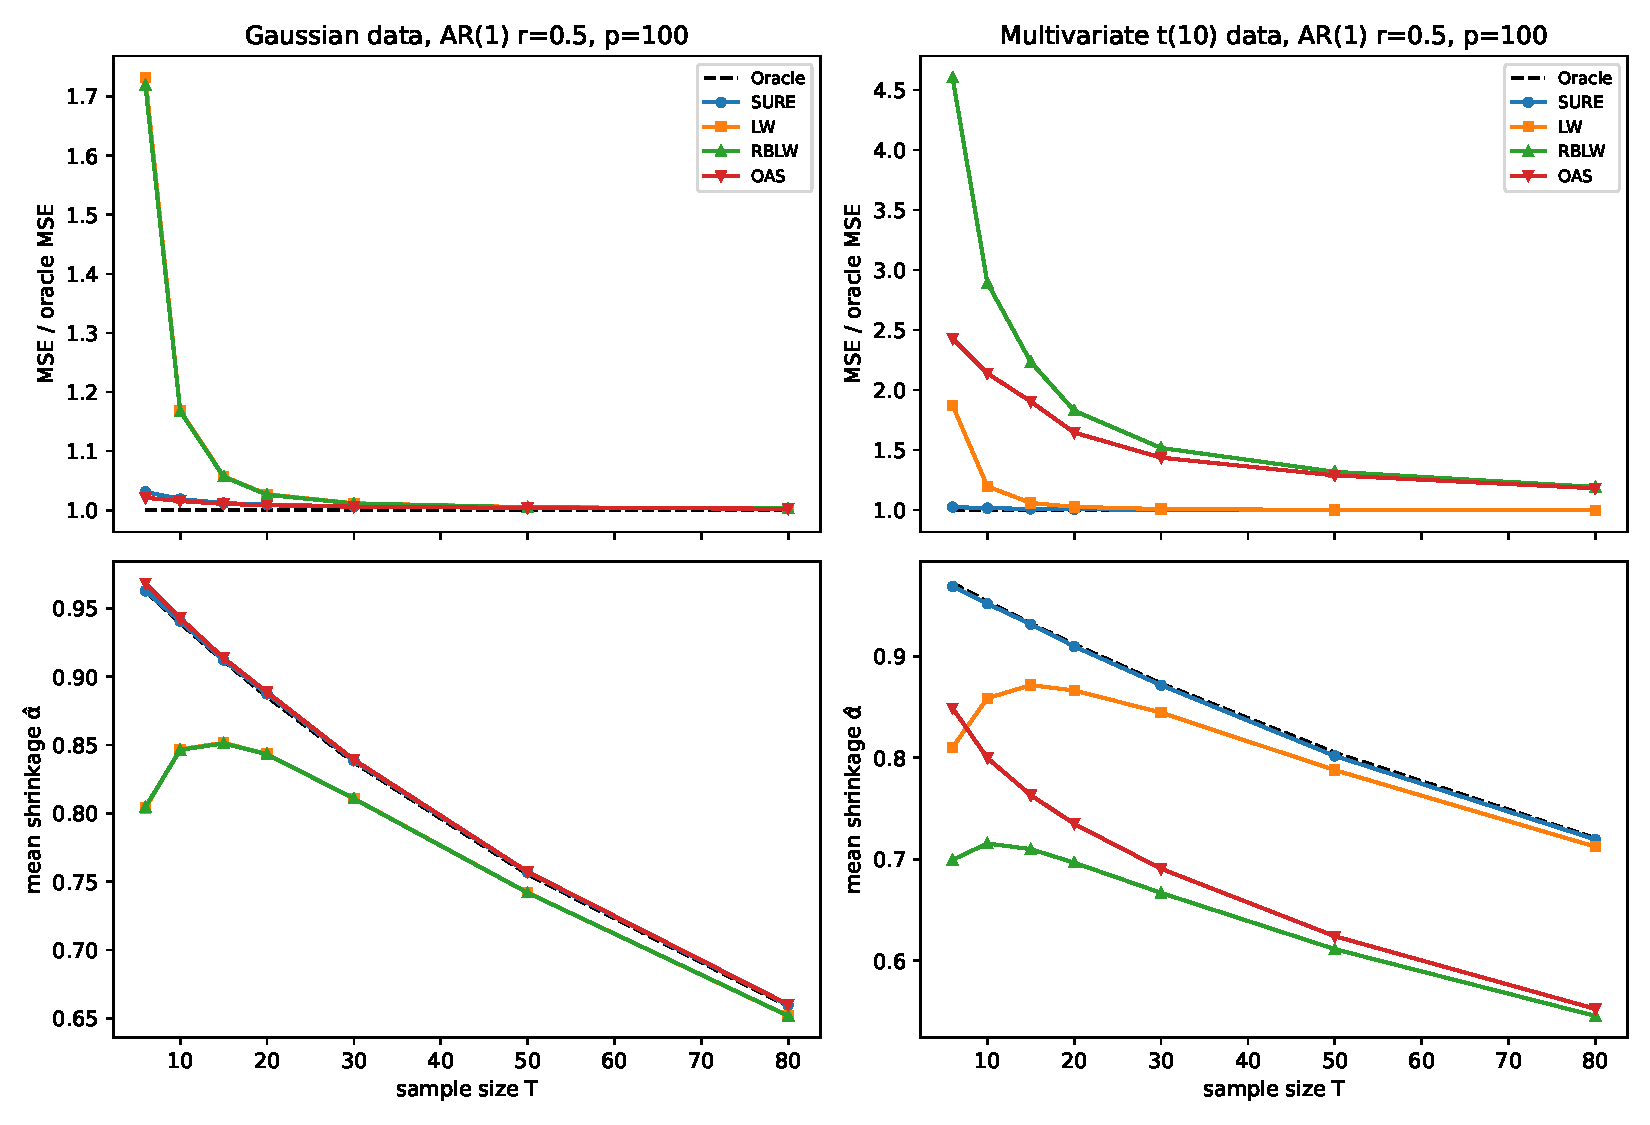
\includegraphics[width=0.49\textwidth]{fig_compare.pdf}
\end{center}
\textit{Left:} SURE$(\delta)$ against the true $R(\delta)$ for $\nu I$ ($p=100$, $T=20$): the mean curve is
within 0.2\% of the truth, the covariance version of the right panel on page 4. \textit{Right:} MSE of
SURE, LW, RBLW, OAS against the oracle. At $T=6$: Gaussian, oracle 63.9, SURE 65.8, LW 110.6; $t_{10}$,
oracle 70.5, SURE 72.2, LW 131.9, RBLW 324.3, OAS 171.1.

\newpage
\section*{Where the work stands}
\begin{enumerate}
\item \textbf{Question} (proposal, Aug 2026): can SURE tune $\delta$, especially for targets with no closed-form $\delta$?
\item \textbf{Literature}: Ledoit \& Wolf (2003, 2004); Yi \& Zou (2013); Chen, Wiesel, Eldar \& Hero (2010); Touloumis (2015).
\item \textbf{Risk in SURE form}: $R(\delta)=\delta^2D+(1-2\delta)V+2\delta C$ (\texttt{sure\_derivation.pdf}).
\item \textbf{Estimating the terms}: exact distribution-free $\hat V,\hat C$ for $F=\nu I$ \newline (\texttt{sure\_scaled\_identity.pdf}).
\item \textbf{Theory}: $R(\delta)<R(0)$ iff $0<\delta<2\delta^*$, and $\delta^*\ge0$. LW is SURE with two finite-sample terms dropped.
\item \textbf{Simulation}: \texttt{stein\_js.py} (page 4) and \texttt{sure\_sim.py} (SURE vs.\ LW, RBLW, OAS).
\item \textbf{Stein map}: every result above has a normal-means counterpart (pages 16--18).
\item \textbf{Open}: choice of target; $S$ with $1/T$ vs.\ $1/(T-1)$; unknown mean; Touloumis comparison; portfolio application.
\end{enumerate}

\section*{References}
\small
Baranchik, A.J. (1964). Multiple regression and estimation of the mean of a multivariate normal
distribution. Technical Report 51, Dept.\ of Statistics, Stanford University.\\
Chen, Y., Wiesel, A., Eldar, Y.C. and Hero, A.O. (2010). Shrinkage algorithms for MMSE covariance
estimation. \textit{IEEE Trans.\ Signal Processing} 58(10).\\
Efron, B. (2004). The estimation of prediction error: covariance penalties and cross-validation.
\textit{JASA} 99(467).\\
Efron, B. and Morris, C. (1973). Stein's estimation rule and its competitors: an empirical Bayes
approach. \textit{JASA} 68(341).\\
Haff, L.R. (1980). Empirical Bayes estimation of the multivariate normal covariance matrix.
\textit{Ann.\ Statist.} 8(3).\\
James, W. and Stein, C. (1961). Estimation with quadratic loss. \textit{Proc.\ Fourth Berkeley Symp.} 1.\\
Ledoit, O. and Wolf, M. (2003). Improved estimation of the covariance matrix of stock returns.
\textit{J.\ Empirical Finance} 10(5).\\
Ledoit, O. and Wolf, M. (2004). A well-conditioned estimator for large-dimensional covariance matrices.
\textit{J.\ Multivariate Anal.} 88(2).\\
Sch\"afer, J. and Strimmer, K. (2005). A shrinkage approach to large-scale covariance matrix estimation
and implications for functional genomics. \textit{Stat.\ Appl.\ Genet.\ Mol.\ Biol.} 4(1).\\
Stein, C. (1981). Estimation of the mean of a multivariate normal distribution. \textit{Ann.\ Statist.} 9(6).\\
Touloumis, A. (2015). Nonparametric Stein-type shrinkage covariance matrix estimators in high-dimensional
settings. \textit{Comput.\ Statist.\ Data Anal.} 83.\\
Yi, F. and Zou, H. (2013). SURE-tuned tapering estimation of large covariance matrices.
\textit{Comput.\ Statist.\ Data Anal.} 58.
\end{document}
